\documentclass[aps,pra,groupedaddress,twocolumn,notitlepage,superscriptaddress,10pt]{revtex4-1}

%\usepackage[utf8]{inputenc}
%\usepackage{mathpazo}
%\usepackage{mathptmx}
%\usepackage{tgpagella}
%\usepackage{tgtermes}

\usepackage{float}
\usepackage{graphicx}  % needed for figures
\usepackage{xcolor}
\usepackage{dcolumn}   % needed for some tables
\usepackage{bm}        % for math
\usepackage{braket}
\usepackage{amssymb}   % for math
\usepackage{epstopdf}
\usepackage{xfrac}

\usepackage{amsmath}
\usepackage{amsthm}
\usepackage{amsfonts}
\usepackage{bbm}
% configure hyperref to remove ugly boxes from links
\definecolor{darkblue}{rgb}{0.1,0.2,0.6}
\definecolor{darkred}{rgb}{0.8,0.1,0.2}
\usepackage[colorlinks,citecolor=darkblue,linkcolor=darkblue,urlcolor=darkblue]{hyperref} 
\usepackage{tikz}
\usepackage{enumerate}
\usepackage{setspace}
\usepackage{url}  % This makes \url work
\usepackage{mathrsfs}

\def\ua{\uparrow}
\def\da{\downarrow}
\newcommand{\rT}{{\rho^{T_2}} }
\newcommand{\rTa}{{\rho^{T_2}_A} }
\newcommand{\rTc}{{\rho^{T_2}} }
\newcommand{\Hi}{\mathcal{H}}
\newcommand{\Ni}{\mathcal{N}}
\newcommand{\C}{\mathbb{C}}
\newcommand{\Z}{\mathbb{Z}}
\newcommand{\R}{\mathbb{R}}
\newcommand{\I}{\mathbb{I}}
\newcommand{\Rp}{{\cal R}_\text{part}}
\newcommand{\sgn}{\text{sign}}

\newcommand{\xv}{\textbf{x}}
\newcommand{\ev}{\textbf{e}}
\newcommand{\iv}{\textbf{i}}
\newcommand{\jv}{\textbf{j}}
\newcommand{\Tr}{\text{Tr}}
\newcommand{\tr}{\text{Tr}}
\newcommand{\del}{\nabla}
\newcommand{\norm}[1]{\left\lVert#1\right\rVert}

\newcommand{\vac}{\ket{0}\bra{0}}
\newcommand{\kvac}{\ket{\text{vac}}}
\newcommand{\bvac}{\bra{\text{vac}}}
\newcommand{\bigket}[1]{ {\big|{#1}\big\rangle} }
\newcommand{\Bigket}[1]{ {\Big|{#1}\Big\rangle} }
\newcommand{\bigbra}[1]{ {\big\langle{#1}\big|} }
\newcommand{\Bigbra}[1]{ {\Big\langle{#1}\Big|} }


\usepackage{tikz}
\usetikzlibrary{positioning}
\usetikzlibrary{patterns}

%\usepackage{tikzit}

\newcommand*{\HS}[1]{\textcolor{blue}{[HS: #1]}}
\newcommand*{\SL}[1]{\textcolor{magenta}{[SL: \textsf{#1}]}}
\newcommand*{\change}[2]{{\color{red}\sout{#1}}{ \color{blue}#2}}

\begin{document}

\title{Entanglement transitions in random pure states}
\author{Hassan Shapourian%
%  \thanks{Electronic address: \texttt{hassan.shapp@gmail.com}}
  }
% \affiliation{Department of Physics, Harvard University, Cambridge, MA~02138, USA}
% \affiliation{Department of Physics, Massachusetts Institute of Technology,
% Cambridge, MA~02139, USA}
\author{Jonah Kudler-flam%
}
% \affiliation{Kadanoff Center for Theoretical Physics, University of Chicago, IL 60637, USA}


\date{\today}

\begin{abstract}
hello
\end{abstract}

\maketitle


Let us look at the dominant diagrams deep in the NPT limit, $L_A\gg L_B$, when one subsystem ($A_1$ or $A_2$) is much larger than the other. 
\begin{align}
    \braket{\Tr \left(\rho^{T_2}\right)^{n_e} } \approx \ 
    \left\{
    \begin{matrix}
    L_{B}^{1-n_e} L_{A_2}^{2-n_e} & \qquad  L_{A_1} \gg L_{A_2}
    \\
    \\
    L_{B}^{1-n_e} L_{A_1}^{2-n_e} & \qquad  L_{A_1} \ll L_{A_2}
    \end{matrix}
    \right.
\end{align}

\begin{align}
    &
    \vcenter{\hbox{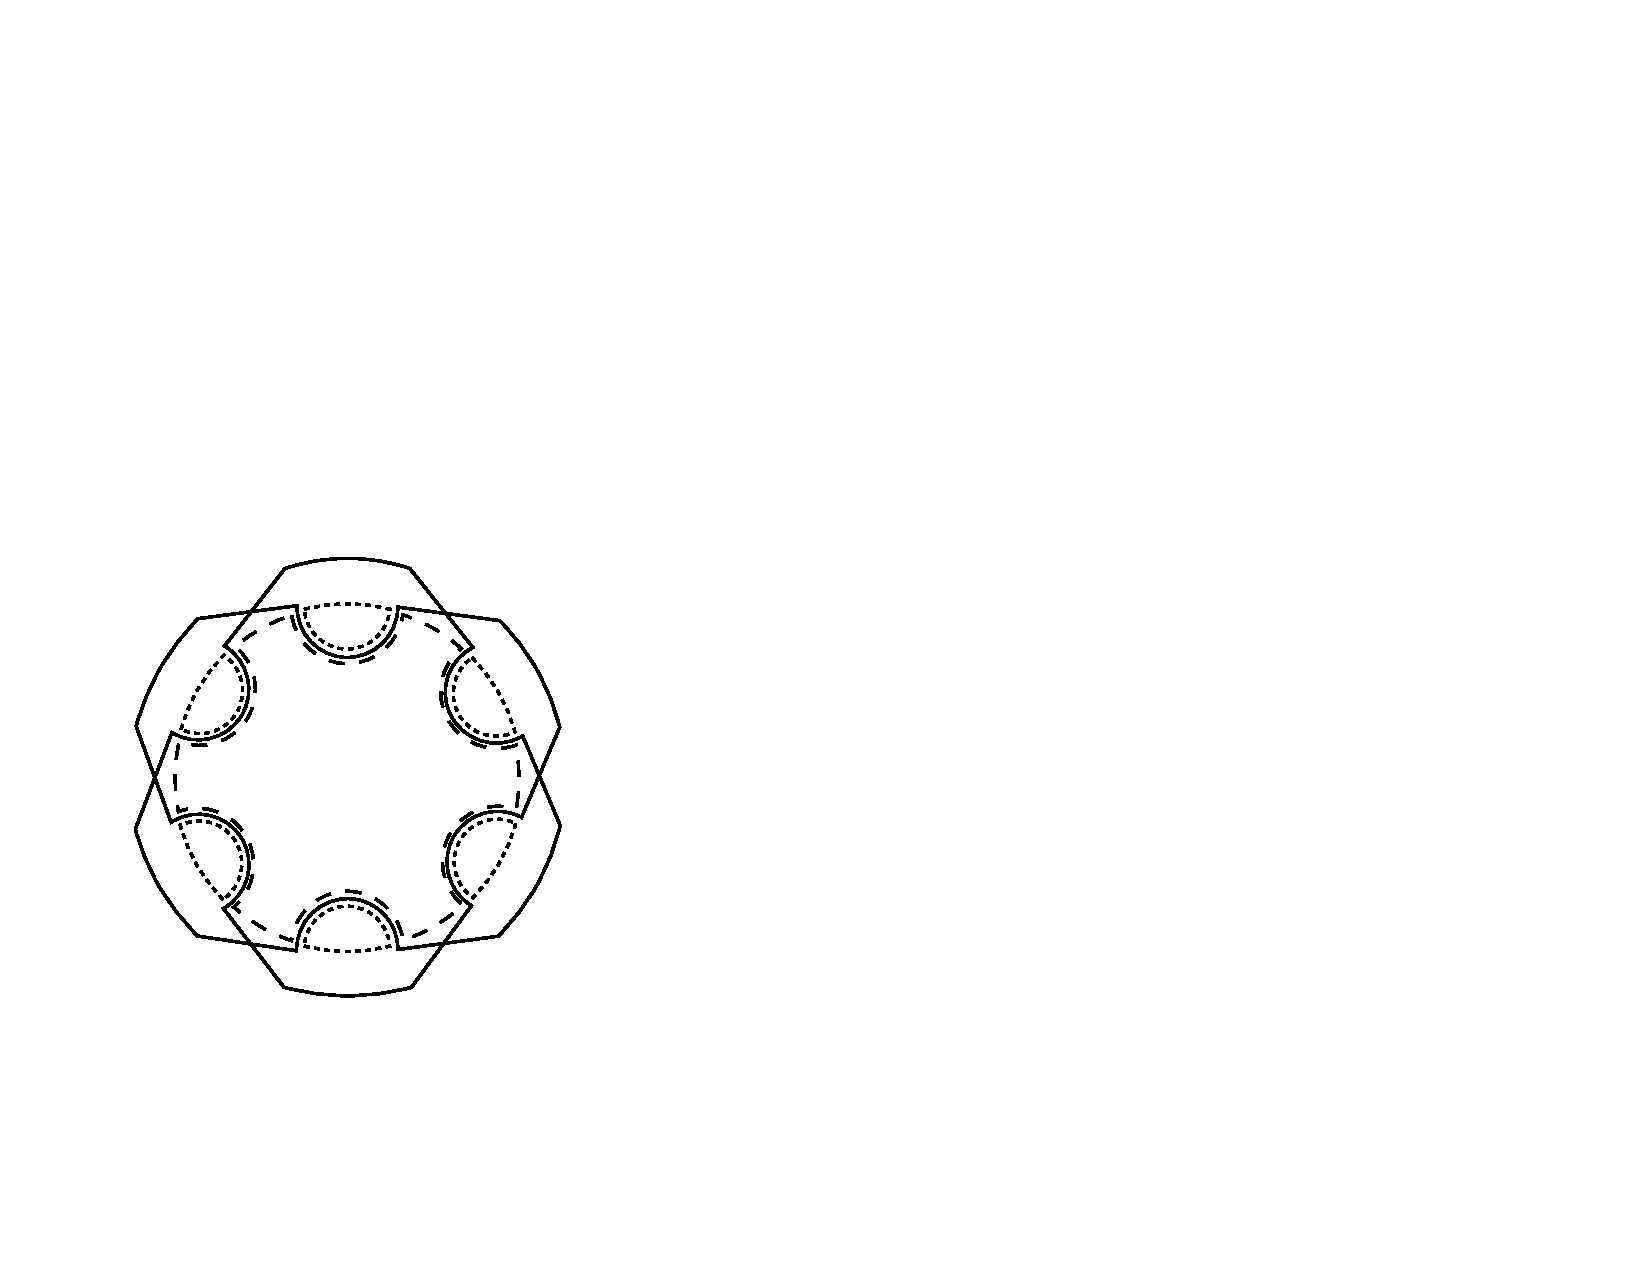
\includegraphics[scale=0.4]{images/RN6_A1large.pdf}}},
\end{align}
\begin{align}
    \vcenter{\hbox{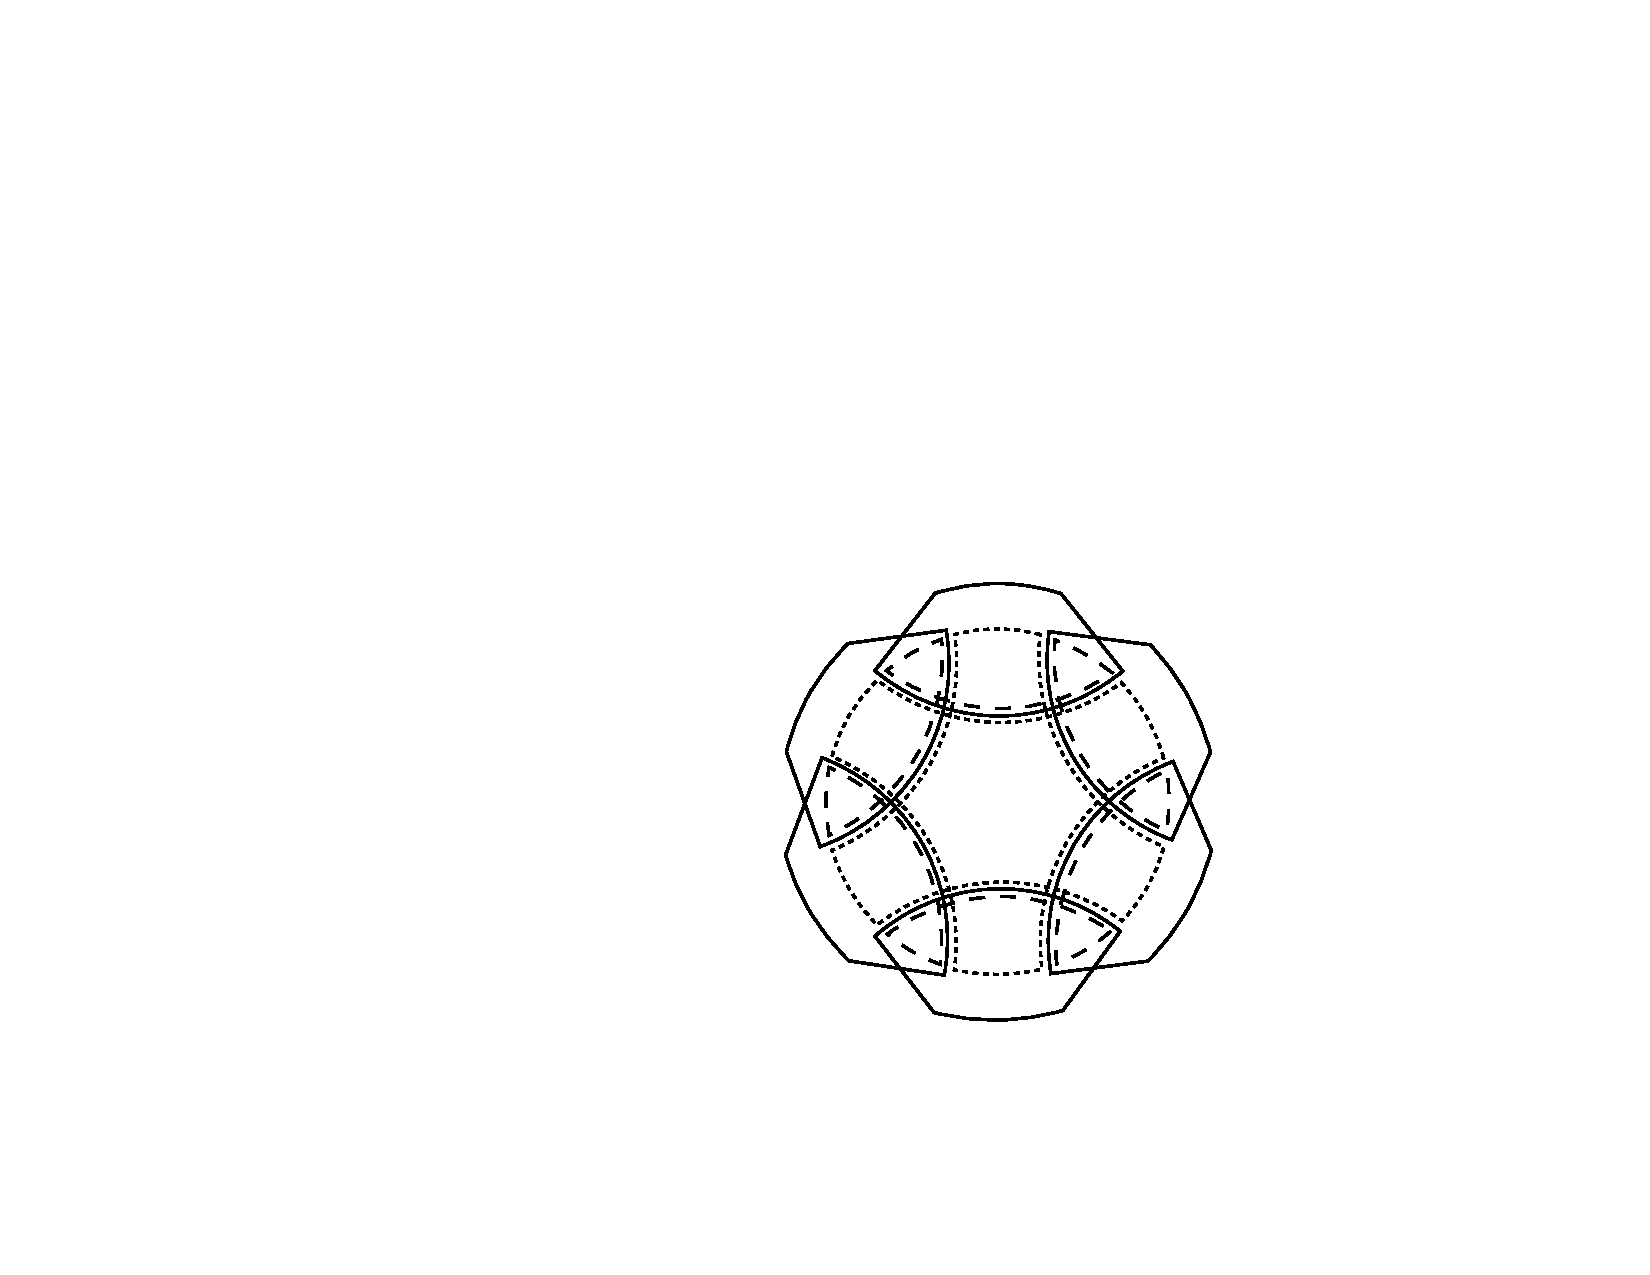
\includegraphics[scale=0.4]{images/RN6_A2large.pdf}}},
\end{align}

To sum up, This in turn implies that
\begin{align}
    \braket{\cal E} \approx \ 
    \left\{
    \begin{matrix}
    L_{B}^{1-n_e} L_{A_2}^{2-n_e} & \qquad  L_{A_1} \gg L_{A_2}
    \\
    \\
    L_{B}^{1-n_e} L_{A_1}^{2-n_e} & \qquad  L_{A_1} \ll L_{A_2}
    \end{matrix}
    \right.
\end{align}

\end{document}